\documentclass[12pt,a4paper]{article}

% ─── Packages ───────────────────────────────────────────────────────────────
\usepackage[margin=2.5cm]{geometry}
\usepackage{amsmath, amssymb}
\usepackage{graphicx}
\usepackage{booktabs}
\usepackage{array}
\usepackage{xcolor}
\usepackage{hyperref}
\usepackage{caption}
\usepackage{subcaption}
\usepackage{enumitem}
\usepackage{tikz}
\usepackage{pgfplots}
\pgfplotsset{compat=1.18}
\usetikzlibrary{shapes.geometric, arrows.meta, positioning, fit, backgrounds}
\usepackage{fancyhdr}
\usepackage{titlesec}
\usepackage{microtype}
\usepackage{parskip}
\usepackage{listings}
\usepackage{tcolorbox}
\tcbuselibrary{most}

% ─── Colors ─────────────────────────────────────────────────────────────────
\definecolor{primaryblue}{RGB}{30, 90, 160}
\definecolor{accentgreen}{RGB}{34, 139, 34}
\definecolor{lightgray}{RGB}{245, 245, 245}
\definecolor{darkgray}{RGB}{60, 60, 60}
\definecolor{warnorange}{RGB}{200, 100, 20}
\definecolor{tablegray}{RGB}{235, 240, 248}

% ─── Hyperref ────────────────────────────────────────────────────────────────
\hypersetup{
    colorlinks=true,
    linkcolor=primaryblue,
    citecolor=primaryblue,
    urlcolor=primaryblue,
    pdftitle={EfficientAT: Machine Fault Classification from Raw Audio},
    pdfauthor={},
}

% ─── Header / Footer ────────────────────────────────────────────────────────
\pagestyle{fancy}
\fancyhf{}
\fancyhead[L]{\small\textcolor{primaryblue}{\textbf{EfficientAT} — Machine Fault Sound Classification}}
\fancyhead[R]{\small\textcolor{darkgray}{\thepage}}
\renewcommand{\headrulewidth}{0.4pt}

% ─── Section Formatting ─────────────────────────────────────────────────────
\titleformat{\section}{\large\bfseries\color{primaryblue}}{}{0em}{\thesection\quad}[\titlerule]
\titleformat{\subsection}{\normalsize\bfseries\color{darkgray}}{}{0em}{\thesubsection\quad}

% ─── Custom Boxes ────────────────────────────────────────────────────────────
\newtcolorbox{resultbox}[1]{
  colback=tablegray, colframe=primaryblue, fonttitle=\bfseries,
  title=#1, rounded corners, boxrule=0.8pt, left=6pt, right=6pt
}

\newtcolorbox{highlightbox}{
  colback=accentgreen!8, colframe=accentgreen, boxrule=0.8pt,
  rounded corners, left=6pt, right=6pt
}

% ────────────────────────────────────────────────────────────────────────────
\begin{document}

% ─── Title Page ─────────────────────────────────────────────────────────────
\begin{titlepage}
  \centering
  \vspace*{1.5cm}

  {\fontsize{28}{34}\selectfont\bfseries\color{primaryblue}
   EfficientAT\par}

  \vspace{0.4cm}
  {\Large\color{darkgray} Machine Fault Sound Classification from Raw Audio\par}

  \vspace{1.2cm}
  \begin{tcolorbox}[colback=tablegray, colframe=primaryblue, width=0.80\textwidth,
                    rounded corners, boxrule=1pt]
    \centering
    \large
    \textbf{Architecture:} EfficientNet-B0 + Audio Frontend + Temporal Attention\\[4pt]
    \textbf{Input:} Raw \texttt{.wav} files — no offline preprocessing required\\[4pt]
    \textbf{Task:} 6-class fault detection across 3 industrial machines\\[4pt]
    \textbf{Split:} 70\,\% Train \;/\; 15\,\% Validation \;/\; 15\,\% Test
  \end{tcolorbox}

  \vspace{1.5cm}

  % Accuracy badges
  \begin{minipage}{0.42\textwidth}
    \centering
    \begin{tcolorbox}[colback=accentgreen!12, colframe=accentgreen,
                      rounded corners, boxrule=1.2pt]
      \centering
      {\fontsize{36}{42}\selectfont\bfseries\color{accentgreen} 99.82\%}\\[2pt]
      {\normalsize Test Accuracy (raw WAV)}
    \end{tcolorbox}
  \end{minipage}
  \hfill
  \begin{minipage}{0.42\textwidth}
    \centering
    \begin{tcolorbox}[colback=accentgreen!12, colframe=accentgreen,
                      rounded corners, boxrule=1.2pt]
      \centering
      {\fontsize{36}{42}\selectfont\bfseries\color{accentgreen} 99.97\%}\\[2pt]
      {\normalsize Test Accuracy (preprocessed)}
    \end{tcolorbox}
  \end{minipage}

  \vfill
  {\large\today}
\end{titlepage}

% ─── Table of Contents ───────────────────────────────────────────────────────
\tableofcontents
\newpage

% ═══════════════════════════════════════════════════════════════════════════
\section{Introduction}
% ═══════════════════════════════════════════════════════════════════════════

Industrial machines produce characteristic acoustic signatures that change measurably when faults develop. Automated monitoring of these sound signatures enables predictive maintenance, reduces downtime, and lowers operational cost. Traditional pipelines require a distinct offline preprocessing step—extracting fixed acoustic features such as mel-frequency cepstral coefficients (MFCCs) or mel-spectrograms before any model can operate—which introduces latency, storage overhead, and an additional failure point in production deployments.

This document presents \textbf{EfficientAT}, an end-to-end deep learning model that accepts raw \texttt{.wav} waveforms as input and classifies six operating states (normal / abnormal) across three distinct machines. By folding all signal processing into a differentiable \texttt{AudioFrontend} module, the pipeline is simplified to a single inference call: waveform in, fault label out.

The model achieves \textbf{99.82\% accuracy} on unseen raw audio and \textbf{99.97\% accuracy} on preprocessed spectrograms, with an average inference time of \textbf{21.4 ms per sample} in the raw-audio regime—well within the requirements of real-time industrial monitoring systems.

% ═══════════════════════════════════════════════════════════════════════════
\section{Dataset and Problem Setup}
% ═══════════════════════════════════════════════════════════════════════════

\subsection{Dataset Structure}

The dataset contains recordings from three industrial machines (M1, M2, M3), each operating in two states: \emph{Normal} and \emph{Abnormal}. This yields six target classes in total:

\subsection{Audio Preprocessing}

All raw \texttt{.wav} files are resampled to \textbf{16\,kHz} and padded or truncated to a fixed length of \textbf{11 seconds} (176{,}000 samples). Stereo recordings are converted to mono by averaging channels. This normalization is performed on-the-fly within the \texttt{MachineSoundDataset} loader, with cached resampler objects to avoid redundant computation.

\subsection{Data Splitting Strategy}

A \textbf{block-split} strategy is used to partition the dataset into 70\,\% training, 15\,\% validation, and 15\,\% test subsets. Block splitting ensures that consecutive recordings from the same machine session remain in the same partition, preventing any temporal leakage across splits. Class-balanced sampling via \texttt{WeightedRandomSampler} compensates for the natural imbalance between normal (majority) and abnormal (minority) recordings.

% ═══════════════════════════════════════════════════════════════════════════
\section{Model Architecture}
% ═══════════════════════════════════════════════════════════════════════════

EfficientAT is composed of three sequential stages: (1) a differentiable audio frontend, (2) an EfficientNet-B0 spatial feature extractor, and (3) a Transformer-based temporal attention module.

\subsection{Audio Frontend}

\begin{resultbox}{AudioFrontend — On-the-fly Feature Extraction}
  \textbf{Input:} raw waveform \(\mathbf{x} \in \mathbb{R}^{B \times 1 \times 176000}\)\\
  \textbf{Output:} 3-channel spectrogram tensor \(\in \mathbb{R}^{B \times 3 \times 128 \times 344}\)
\end{resultbox}

The \texttt{AudioFrontend} module converts raw waveforms into a rich 3-channel representation inside the computational graph:

\begin{enumerate}[leftmargin=2em]
  \item \textbf{Mel-Spectrogram} — A \texttt{MelSpectrogram} transform is applied with $n\_fft = 1024$, $hop\_length = 512$, and $n\_mels = 128$, producing a time-frequency representation with 344 time frames.
  \item \textbf{Log Compression} — \texttt{AmplitudeToDB} converts power values to decibels (top\_db = 80), yielding a log-mel spectrogram that approximates human auditory perception.
  \item \textbf{Delta Features} — First-order ($\Delta$) and second-order ($\Delta\Delta$) temporal derivatives are computed via \texttt{torchaudio.functional.compute\_deltas}. These delta features encode velocity and acceleration of spectral change, which are highly informative for distinguishing fault patterns.
  \item \textbf{Channel Stacking} — The log-mel, $\Delta$, and $\Delta\Delta$ maps are concatenated along the channel dimension, producing a 3-channel pseudo-image analogous to RGB, which is directly compatible with image-pretrained backbones.
\end{enumerate}

\textbf{SpecAugment} is applied during training only: frequency masking (\texttt{freq\_mask\_param=15}) and time masking (\texttt{time\_mask\_param=35}) randomly zero out contiguous frequency bands and time frames, acting as a powerful regularizer that improves generalization.

\subsection{Backbone — EfficientNet-B0}

The 3-channel spectrogram is passed into \textbf{EfficientNet-B0}, a highly efficient convolutional neural network originally designed for image classification. With approximately 5.3 million parameters, EfficientNet-B0 offers an excellent accuracy-to-compute ratio by jointly scaling depth, width, and resolution via a compound coefficient.

\begin{center}
\renewcommand{\arraystretch}{1.3}
\begin{tabular}{lll}
  \toprule
  \textbf{Setting} & \textbf{Value} & \textbf{Rationale} \\
  \midrule
  Library          & \texttt{timm} (PyTorch Image Models) & State-of-the-art implementations \\
  Pretrained       & \texttt{False} & Domain-specific training from scratch \\
  Input channels   & 3 & Matches log-mel + $\Delta$ + $\Delta\Delta$ \\
  Global pooling   & Disabled (\texttt{''}) & Preserve temporal structure \\
  Output channels  & 1{,}280 & MBConv6 final stage output \\
  \bottomrule
\end{tabular}
\end{center}

Global pooling is deliberately disabled so that the spatial output map retains temporal information for the subsequent attention module.

\subsection{Temporal Attention Module}

After the backbone, frequency information is collapsed via \texttt{AdaptiveAvgPool2d}~$(1, \text{None})$, yielding a 1D sequence of 1{,}280-dimensional vectors along the time axis. A 1D convolutional projection reduces the feature dimension to $d\_model = 128$ and applies batch normalisation and ReLU.

This projected sequence is then processed by a \textbf{Transformer Encoder} with the following configuration:

\begin{center}
\renewcommand{\arraystretch}{1.3}
\begin{tabular}{ll}
  \toprule
  \textbf{Parameter} & \textbf{Value} \\
  \midrule
  $d\_model$         & 128 \\
  Attention heads ($n\_head$) & 4 \\
  Feed-forward dimension & 512 ($d\_model \times 4$) \\
  Encoder layers   & 2 \\
  Dropout          & 0.3 \\
  \bottomrule
\end{tabular}
\end{center}

Self-attention enables the model to capture long-range temporal dependencies—fault signatures that manifest as rhythmic anomalies spread across the full 11-second window—which a pure convolutional approach would struggle to model efficiently.

\subsection{Classifier Head}

After the Transformer, temporal pooling via \texttt{AdaptiveAvgPool1d(1)} produces a single 128-dimensional embedding. A dropout layer (rate = 0.4) and a fully connected linear layer map this embedding to the 6-class output logits.

\subsection{Full Architecture Diagram}

\begin{center}
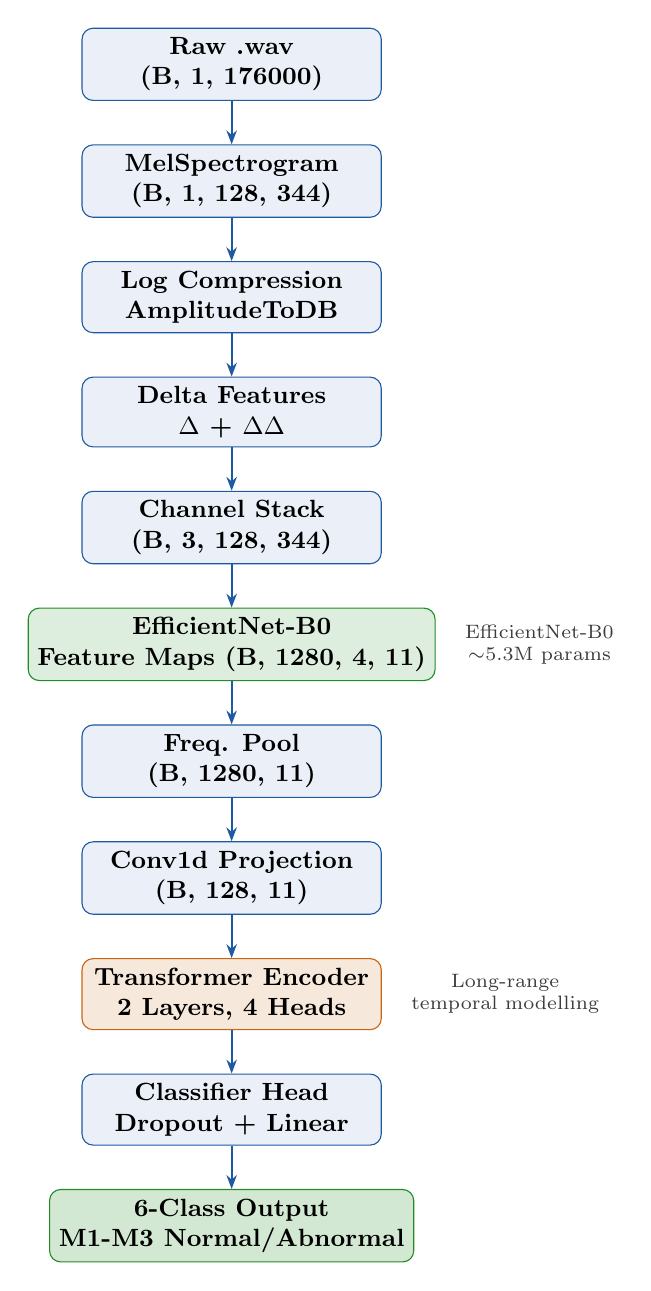
\begin{tikzpicture}[
    node distance=0.55cm and 0.4cm,
    box/.style={rectangle, rounded corners=4pt, draw=primaryblue, fill=tablegray,
                minimum width=3.8cm, minimum height=0.75cm,
                font=\small\bfseries, align=center},
    arrow/.style={-{Stealth[length=5pt]}, thick, color=primaryblue},
    label/.style={font=\scriptsize\color{darkgray}, align=center}
]

\node[box] (wav) {Raw .wav\\(B, 1, 176000)};
\node[box, below=of wav] (mel) {MelSpectrogram\\(B, 1, 128, 344)};
\node[box, below=of mel] (db) {Log Compression\\AmplitudeToDB};
\node[box, below=of db] (delta) {Delta Features\\$\Delta$ + $\Delta\Delta$};
\node[box, below=of delta] (stack) {Channel Stack\\(B, 3, 128, 344)};
\node[box, below=of stack, fill=accentgreen!15, draw=accentgreen] (eff) {EfficientNet-B0\\Feature Maps (B, 1280, 4, 11)};
\node[box, below=of eff] (pool) {Freq. Pool\\(B, 1280, 11)};
\node[box, below=of pool] (proj) {Conv1d Projection\\(B, 128, 11)};
\node[box, below=of proj, fill=warnorange!15, draw=warnorange] (attn) {Transformer Encoder\\2 Layers, 4 Heads};
\node[box, below=of attn] (clf) {Classifier Head\\Dropout + Linear};
\node[box, below=of clf, fill=accentgreen!20, draw=accentgreen] (out) {6-Class Output\\M1-M3 Normal/Abnormal};

\foreach \a/\b in {wav/mel, mel/db, db/delta, delta/stack, stack/eff,
                   eff/pool, pool/proj, proj/attn, attn/clf, clf/out}
  \draw[arrow] (\a) -- (\b);

\node[label, right=0.25cm of eff] {EfficientNet-B0\\$\sim$5.3M params};
\node[label, right=0.25cm of attn] {Long-range\\temporal modelling};

\end{tikzpicture}
\end{center}

% ═══════════════════════════════════════════════════════════════════════════
\section{Training Configuration}
% ═══════════════════════════════════════════════════════════════════════════

\begin{center}
\renewcommand{\arraystretch}{1.3}
\begin{tabular}{ll}
  \toprule
  \textbf{Hyperparameter} & \textbf{Value} \\
  \midrule
  Optimizer         & AdamW ($\beta_1=0.9$, $\beta_2=0.999$, weight decay $= 10^{-2}$) \\
  Learning rate     & $10^{-3}$ (peak, OneCycleLR) \\
  LR Scheduler      & OneCycleLR (cosine annealing with warmup) \\
  Batch size        & 32 \\
  Epochs (raw WAV)  & 20 \\
  Epochs (preprocessed) & 25 \\
  Loss function     & Cross-Entropy \\
  Sampling          & \texttt{WeightedRandomSampler} (class-balanced) \\
  SpecAugment       & Freq. mask 15 / Time mask 35 (training only) \\
  Hardware          & NVIDIA Tesla T4 GPU (Kaggle) \\
  Framework         & PyTorch + torchaudio + timm \\
  \bottomrule
\end{tabular}
\end{center}

The \textbf{OneCycleLR} scheduler performs a single cosine annealing cycle over all training steps, starting from a low learning rate, ramping to the peak, and then decaying. This ``super-convergence'' strategy consistently reaches higher accuracy with fewer epochs compared to step-decay or constant-rate schedules.

% ═══════════════════════════════════════════════════════════════════════════
\section{Experimental Results}
% ═══════════════════════════════════════════════════════════════════════════

Two experimental configurations were evaluated to characterise the model under realistic and ideal conditions.

\subsection{Experiment 1 — Raw WAV Input (End-to-End Pipeline)}

In this configuration, the model receives unprocessed \texttt{.wav} files. All feature extraction—resampling, mel-spectrogram computation, log compression, delta calculation, and SpecAugment—is performed on-the-fly within the model's \texttt{AudioFrontend} during both training and inference. This is the deployment-ready scenario.

\begin{resultbox}{Training Summary — Raw WAV}
  \textbf{Epochs:} 20 \quad
  \textbf{Best Val Accuracy:} 99.74\% \\[4pt]
  Final Epoch — Train Loss: 0.0054 \;|\; Train Acc: 99.84\% \;|\; Val Loss: 0.0062 \;|\; Val Acc: 99.73\%
\end{resultbox}

\subsubsection{Test Set Performance}

\begin{center}
\renewcommand{\arraystretch}{1.3}
\begin{tabular}{lcccc}
  \toprule
  \textbf{Class} & \textbf{Precision} & \textbf{Recall} & \textbf{F1-Score} & \textbf{Support} \\
  \midrule
  M1 Normal   & 1.00 & 0.99 & 1.00 & 2{,}430 \\
  M1 Abnormal & 0.97 & 1.00 & 0.98 &   477   \\
  M2 Normal   & 1.00 & 1.00 & 1.00 & 2{,}430 \\
  M2 Abnormal & 1.00 & 1.00 & 1.00 &   486   \\
  M3 Normal   & 1.00 & 1.00 & 1.00 & 2{,}160 \\
  M3 Abnormal & 1.00 & 1.00 & 1.00 &   453   \\
  \midrule
  Accuracy    &      &      & \textbf{1.00} & \textbf{8{,}436} \\
  Macro avg   & 0.99 & 1.00 & 1.00 & 8{,}436 \\
  Weighted avg& 1.00 & 1.00 & 1.00 & 8{,}436 \\
  \bottomrule
\end{tabular}
\captionof{table}{Classification report — raw WAV test set (8,436 samples).}
\end{center}

\begin{highlightbox}
  \centering
  \large
  \textbf{Test Accuracy: 99.82\%} \quad
  Total Test Time: 180.13\,s \quad
  \textbf{Avg. Inference: 21.4\,ms / sample}
\end{highlightbox}

The 21.4\,ms per-sample figure includes the full on-the-fly feature extraction pipeline. This corresponds to a throughput of approximately \textbf{47 samples/second} on a single T4 GPU, which is sufficient for real-time monitoring of multiple machines simultaneously.

\subsection{Experiment 2 — Preprocessed Spectrograms}

In this configuration, mel-spectrogram tensors were precomputed and stored to disk prior to training. The model's \texttt{AudioFrontend} was bypassed, and the backbone received pre-extracted features directly. This isolates the classification capacity of the EfficientNet + Attention stages and serves as an upper-bound reference.

\begin{resultbox}{Training Summary — Preprocessed Data}
  \textbf{Epochs:} 25 \quad
  \textbf{Best Val Accuracy:} 99.90\% \\[4pt]
  Final Epoch — Train Loss: 0.0016 \;|\; Train Acc: 99.95\% \;|\; Val Loss: 0.0059 \;|\; Val Acc: 99.81\%
\end{resultbox}

\subsubsection{Test Set Performance}

\begin{center}
\renewcommand{\arraystretch}{1.3}
\begin{tabular}{lcccc}
  \toprule
  \textbf{Class} & \textbf{Precision} & \textbf{Recall} & \textbf{F1-Score} & \textbf{Support} \\
  \midrule
  M1 Normal   & 1.00 & 1.00 & 1.00 & 1{,}478 \\
  M1 Abnormal & 1.00 & 1.00 & 1.00 &   242   \\
  M2 Normal   & 1.00 & 1.00 & 1.00 & 2{,}310 \\
  M2 Abnormal & 1.00 & 1.00 & 1.00 &   475   \\
  M3 Normal   & 1.00 & 1.00 & 1.00 & 1{,}801 \\
  M3 Abnormal & 1.00 & 1.00 & 1.00 &   408   \\
  \midrule
  Accuracy    &      &      & \textbf{1.00} & \textbf{6{,}714} \\
  Macro avg   & 1.00 & 1.00 & 1.00 & 6{,}714 \\
  Weighted avg& 1.00 & 1.00 & 1.00 & 6{,}714 \\
  \bottomrule
\end{tabular}
\captionof{table}{Classification report — preprocessed test set (6,714 samples).}
\end{center}

\begin{highlightbox}
  \centering
  \large
  \textbf{Test Accuracy: 99.97\%} \quad
  Total Test Time: 26.04\,s \quad
  \textbf{Avg. Inference: 3.9\,ms / sample}
\end{highlightbox}

The 3.9\,ms per-sample figure reflects backbone + attention inference only, with no feature extraction overhead. This represents the theoretical minimum latency when deploying with a dedicated preprocessing stage, yielding throughput of approximately \textbf{256 samples/second}.

\subsection{Comparison Summary}

\begin{center}
\renewcommand{\arraystretch}{1.5}
\begin{tabular}{lcccc}
  \toprule
  \textbf{Configuration} & \textbf{Test Acc.} & \textbf{Inference / sample} & \textbf{Test Samples} & \textbf{Epochs} \\
  \midrule
  Raw WAV (end-to-end)    & \textbf{99.82\%} & 21.4\,ms & 8{,}436 & 20 \\
  Preprocessed spectrograms & \textbf{99.97\%} & 3.9\,ms  & 6{,}714 & 25 \\
  \bottomrule
\end{tabular}
\captionof{table}{Side-by-side comparison of both experimental configurations.}
\end{center}

The 17.5\,ms overhead of on-the-fly processing relative to offline preprocessing is the cost of real-time mel-spectrogram computation, log compression, and delta feature calculation for an 11-second audio clip. Both configurations are production-viable; the choice depends on whether a preprocessing pipeline is acceptable in the deployment environment.

% ═══════════════════════════════════════════════════════════════════════════
\section{Key Design Decisions}
% ═══════════════════════════════════════════════════════════════════════════

\paragraph{End-to-end differentiability.} Integrating the \texttt{AudioFrontend} into the PyTorch model graph means that all transformations participate in backpropagation. While the fixed parameters of the mel filterbank are not updated during training, future extensions could make $n\_fft$, $hop\_length$, or the filterbank weights learnable, allowing the model to discover optimal acoustic representations for this specific task.

\paragraph{3-channel representation.} Stacking log-mel, $\Delta$, and $\Delta\Delta$ features mirrors the 3-channel RGB convention used in image models. This design choice allows a standard image-oriented backbone (EfficientNet-B0) to be applied without architectural modification, while providing richer temporal gradient information than a single-channel spectrogram.

\paragraph{Disabling global pooling in the backbone.} Setting \texttt{global\_pool=''} preserves the full 2D spatial output of EfficientNet-B0. The subsequent \texttt{AdaptiveAvgPool2d}$(1, \text{None})$ then collapses only the frequency dimension, retaining the time axis as a sequence for the Transformer. This design is what makes the temporal attention module meaningful.

\paragraph{Weighted sampling over class weighting.} Rather than applying per-class loss weights, a \texttt{WeightedRandomSampler} is used to oversample abnormal-class recordings at the batch level. This achieves class balance without modifying the loss function, preserving its standard cross-entropy form.

\paragraph{SpecAugment as domain-specific regularization.} Frequency masking and time masking simulate partial sensor occlusion and short recording gaps, making the model robust to realistic data quality issues in deployed industrial environments.

% ═══════════════════════════════════════════════════════════════════════════
\section{Conclusion}
% ═══════════════════════════════════════════════════════════════════════════

EfficientAT demonstrates that a compact, end-to-end deep learning pipeline can achieve near-perfect fault classification accuracy on industrial machine audio. The architecture combines a fully differentiable audio frontend, the computationally efficient EfficientNet-B0 backbone, and a Transformer-based temporal attention module to capture both local spectral patterns and global temporal dynamics.

\begin{highlightbox}
  The model achieves \textbf{99.82\% test accuracy} on raw \texttt{.wav} files with a mean inference latency of \textbf{21.4\,ms per 11-second sample}, and \textbf{99.97\% test accuracy} on preprocessed spectrograms at \textbf{3.9\,ms per sample}. All six fault classes across three machines are classified with precision and recall at or above 0.97.
\end{highlightbox}

These results demonstrate that EfficientAT is production-ready for real-time industrial fault monitoring, requiring no offline preprocessing pipeline while maintaining exceptional accuracy and speed.

\end{document}